% uw-wkrpt-ece.tex - An example work report that uses uw-wkrpt.cls
% Copyright (C) 2002,2003  Simon Law
% 
% This program is free software; you can redistribute it and/or modify
% it under the terms of the GNU General Public License as published by
% the Free Software Foundation; either version 2 of the License, or
% (at your option) any later version.
% 
% This program is distributed in the hope that it will be useful,
% but WITHOUT ANY WARRANTY; without even the implied warranty of
% MERCHANTABILITY or FITNESS FOR A PARTICULAR PURPOSE.  See the
% GNU General Public License for more details.
% 
% You should have received a copy of the GNU General Public License
% along with this program; if not, write to the Free Software
% Foundation, Inc., 59 Temple Place, Suite 330, Boston, MA  02111-1307  USA
%
%%%%%%%%%%%%%%%%%%%%%%%%%%%%%%%%%%%%%%%%%%%%%%%%%%%%%%%%%%%%%%%%%%%%%

\documentclass[ece]{uw-wkrpt}

\usepackage{graphicx} % Include graphic importing
\usepackage{algorithm}
\usepackage[noend]{algpseudocode}
\usepackage[table]{xcolor}% http://ctan.org/pkg/xcolor
\usepackage{titlesec}
\usepackage{caption}

\setcounter{secnumdepth}{4}
\setcounter{tocdepth}4

\titleformat{\paragraph}
{\normalfont\normalsize\bfseries}{\theparagraph}{1em}{}
\titlespacing*{\paragraph}
{0pt}{3.25ex plus 1ex minus .2ex}{1.5ex plus .2ex}

\definecolor{mygray}{gray}{0.9}

\let\oldsection\section
\renewcommand\section{\clearpage\oldsection}

\begin{document}

%%%%%%%%%%%%%%%%%%%%%%%%%%%%%%%%%%%%%%%%%%%%%%%%%%%%%%%%%%%%%%%%%%%%%
%% IMPORTANT INFORMATION
%%%%%%%%%%%%%%%%%%%%%%%%%%%%%%%%%%%%%%%%%%%%%%%%%%%%%%%%%%%%%%%%%%%%%

\title{Final Design Report}
\group{Group 12:}
\author{Daniel Dworakowski}
\uwid{Rae Jeong}
\email{Nhat Le}
\authortwo{Ji-Won Park}
\authorthree{Fan Zhang}
\employer{MTE 380 – Mechatronics Engineering Design Workshop}
\school{University of Waterloo}
\faculty{Mechatronics Engineering}
\term{3B}
\program{Mechatronics Engineering}
\address{University of Waterloo,\\*
        Waterloo, ON\ \ N2L 3G1}
\employeraddress{}
\chair{Dr. Bill Owen}
\chairaddress{University of Waterloo,\\*
        Waterloo, ON\ \ N2L 3G1}
\maketitle

%%%%%%%%%%%%%%%%%%%%%%%%%%%%%%%%%%%%%%%%%%%%%%%%%%%%%%%%%%%%%%%%%%%%%
%% FRONT MATTER
%%%%%%%%%%%%%%%%%%%%%%%%%%%%%%%%%%%%%%%%%%%%%%%%%%%%%%%%%%%%%%%%%%%%%
\frontmatter

% 
% Fan.
\begin{letter}
Group 12, consisting of D. Dworakowski, R. Jeong, N. Le, J. Park, F. Zhang, is submitting this report for review.

Members are responsible to work collaboratively and competitively, applying the design process to fulfill the project’s goal. The goal this term involves designing and building a device to go over a wall and delivering a package. This report outlines the major changes that were made as compared to the previous report. Moreover, the design exploration of how these changes came to fruition as well as the tradeoffs that were made when deciding on the final design is talked about inside the report. This leads to an analysis of the performance of the system, as well as how these changes impacted the performance of the robot overall.

As mentioned in the previous report, the group aimed to study and apply the design process in a multidisciplinary environment. The success in the competition and overall completion of the course can be attributed to the application of knowledge from the several courses the group has taken. The experience has significantly improved the inter-personal, leadership and teamwork skills in the team. This experience ultimately serves as an excellent basis for the upcoming forth year design project. 

Group 12 believes that this project provides an opportunity to gain the skills required to be an effective engineer. To that end, all the students in group 12 are aware of the University of Waterloo\textsc{\char13}s academic integrity policy 71 regarding \textsc{\char13}student discipline\textsc{\char13} and have been and will be following it throughout this project. Non-original ideas will be credited and cited to the original author.

\end{letter}
% 
% Fan.
\section{Executive Summary}\label{sec:summary}
\onehalfspacing
Citizens live in the region between the inner and outer walls, making them vulnerable to attacks from monsters beyond the wall. The inner city needs a safe, efficient, and autonomous method to deliver supplies over a wall to those in need in case of emergency.

This report outlines the critical decision making and final design overview of the device that was built to solve this problem. The report provides an analysis and an explanation of the major decisions that were made as compared to the previous report. Overall, the major components of the system that are described are focused on the mechanical, electrical and control engineering. The combination of these components is examined from a high-level to analyze the final results of the competition and any differences in the expected performance. 

Based on the bill of materials, the final cost of the project was around the projected budget of 500 Canadian dollars. The overall project management is analyzed to determine whether the distribution was effective in solving the overall task. This is achieved by analyzing the progress that was made throughout the project and how the project targets influenced the final results.  

Overall, the project was successful in completing in the task that was specified and did so in 52 seconds at 2.4 kilograms of mass. The experimentation and design procedures that were used act as an excellent precursor to the fourth year design project.

\tableofcontents
\listoffigures
\listoftables

%%%%%%%%%%%%%%%%%%%%%%%%%%%%%%%%%%%%%%%%%%%%%%%%%%%%%%%%%%%%%%%%%%%%%
%% REPORT BODY
%%%%%%%%%%%%%%%%%%%%%%%%%%%%%%%%%%%%%%%%%%%%%%%%%%%%%%%%%%%%%%%%%%%%%


\mainmatter

% 
% Rae
\section{Introduction and Background}

The following section describes the purpose of the project. It defines the constraints and criteria of the design, which resulted in a decision to create a robot capable of jumping. It also presents a review of the design’s performance from the competition. 


\subsection{General Background}

Mutant humanoid giants known as titans first appeared on Earth over 100 years ago. They prey upon humans using their strength and speed, and have since then driven humankind into walled cities meant to keep titans out. One of such cities employed an inner and outer wall to fortify its defenses and protect vital city infrastructure located inside the inner walls in the case of a breach. Unfortunately, this meant that most citizens had to live in the area less safe area, between the inner and outer walls.

The city government recognized that the evacuation time of the residents living between the two walls would take long; in the case titans breach the wall. The military will eventually contain the breach and drive the titans back out. However, such an operation may take days. Thus, it was necessary to devise a method to deliver supplies to shelters from the inner city, over the inner wall (as the gate cannot be opened), in a time of need.

The ideal solution should be autonomous, as the mission is highly dangerous and should refrain from risking human lives. It should also be small and stealthy, to minimize the chance of detection by the titans (an aerial solution is therefore out of the question).


\subsection{Problem Formulation}

The following section will describe the problem, the functionality desired of the final design. Objectives, constraints and criteria will be presented to guide the design process and selection.

\subsubsection{Problem Definition}

Design a device to deliver a package from inside the inner walls to shelters in the outer areas.

\subsubsection{Desired Functions and Goals}

The main function of the device is to autonomously identify and navigate to tall poles used by shelters to indicate their location to deliver supplies. The device should be able to overcome tall obstacles in its path.

\subsubsection{Constraints}

The starting size of the device must be smaller than 0.6 m in all dimensions. It must operate autonomously using only its onboard computing power. Without human control and/or influence, the device must be able to complete the mission as defined by the problem statement while staying within the perimeter of the course. To complete the mission, the device must overcome thin, but tall, obstacles up to 0.9 m in height. It cannot accomplish this by burrowing underneath the obstacle, navigating around the obstacle, or through sustained flight.

\subsubsection{Objectives}

The device should be less than 1.5 kg to minimize any risk of injury it poses on humans around it. The device should withstand impacts and resist wear and tear for a minimum of 100 cycles of normal operations without maintenance or repair. If a part were to break, it should be easily replaceable with off the shelf components. Furthermore, the autonomous device should not have more than 10 custom made machined parts. For ease of development, the devices should be tetherable to a computer or external power source while testing for data transfer and/or power. The on-board battery should provide the device with an operational time of at least 10 minutes. Furthermore, the rescue mission should take no longer than 5 minutes. The battery should also be replaceable without the use of tools. The total expenditure for sourcing component should be under \$500 CAD. 

\subsubsection{Design Selection Criteria}

The most important criteria for evaluating a design are the performance index and reliability of the design. The reliability of the device is defined as the number of successful deliveries completed by a design before requiring major repairs or replacement of parts. The performance index (PI), which is a function of criteria mass (m) and time to complete a delivery (t), as shown below.

\[PI = \frac{F_f}{mt^2}\]

The effect of an increase in delivery time on the degradation of the performance index is quadratic. Therefore, time has more significance over mass. This measurement will determine the success of the project relative to competition. Other criteria include ease of repair by replacing components, ease of development, and cost. The full list of criteria is shown in Table \ref{tab:designSelection}. 


\begin{table}[]
\centering
\caption[Performance of the design, along with the corresponding weights]
{Performance of the design, along with the corresponding weights.}
\begin{tabular}{ | l | p{4in} | l |}
\hline
Criteria & Unit & Weight \\ \hline
Cost & Dollars, lower is better & 10 \\ \hline
Mass & Grams, lower is better & 15 \\ \hline
Time to deliver & Seconds, lower is better & 25 \\ \hline
Ease of Repair/Modularity & Rating between 0 and 15, higher is better & 15 \\ \hline
Reliability & Number of trials until repair or maintenance, higher is better & 25 \\ \hline
Ease of Development & Downtime between trials in minutes, lower is better & 10 \\ \hline
\end{tabular}
\label{tab:designSelection}
\end{table}


The most important criteria are time to deliver and reliability, because they are critical qualities the robot must have these to complete the mission. The next most important criteria are the mass and ease of repair. The least important criteria, given weights of 10, are the cost and ease of development. These are nice-to-haves and do not affect the design’s ability to complete the mission.

\subsection{Review of the Selected Design}

One major design problem is the method to overcome obstacles. For a jumping approach, the robot must generate or store sufficient energy to make the 0.9 m jump. This requires a sizable mechanism which increases the robot’s weight, which further increases the energy requirements. In addition, the rapid release of potential energy may damage the mechanism through impact loading. Thus, it is critical to design energy storage and release mechanism that is both minimal and lightweight, but also resistant to impact loading. During the competition, it was observed that the latching mechanism became less reliable because of ware from constant testing. While unexpected the outcome was understandable due to the high forces and significant testing performed using the platform. Moreover, the calculations were performed using an estimate of 1.5 kg for the robot's mass but in reality, the robot was measure to be closer to 2.4 kg. To combat this, additional springs had to be added to the original design to increase the potential energy. More details about the modifications and problems with the jumping mechanism will be presented in Section \ref{mech}.

Although a fall from about a meter in height is not especially damaging mechanically, its effect on delicate electronic components and sensors must be considered. The tradeoff is between using stronger, but heavier, metallic materials or weaker, but lighter, composite materials for the chassis. The design of the chassis, placement of the electronic components and sensors, as well as padding must work in conjunction to protect all components from landing impact. During the competition, while some parts came loose over time, the fall didn’t damage any parts. The bearing arrangement held up very well and only damage that was not anticipated were the wheel shaft deformation. Further details describing issues involving electrical design will be covered in Section \ref{electrical}.

Another major design problem is autonomously locating the destination. The size and computing power constraints for the robot limits the quality and reliability of data available for navigation. The operation of the robot and the environment may introduce noise, which must also be accounted for. A known landing position is therefore desired to help minimize the complexity of the destination location algorithm. Several parameters required tuning to ensure reliability of both driving and finding the destination. Details about the modifications are covered in Section \ref{controls}. 

\section{Project Management}
The following section analyzes how the project progressed throughout the scheduled time as well as a cost analysis and bill of materials of the all components.

\subsection{Schedule}

The schedule of progress can be seen in Figure \ref{fig:gantt} below. In general between the period of time of the second report and the competition date the schedule was generally followed. However, there were some areas which took longer than anticipated, such as software development, manufacturing and construction. Although the core interface for controlling the robot was complete ahead of time, modifications were required to accommodate physical changes to the robot. Similarly, due to changes in the mechanical design construction time was also allotted. Blue cells represent soft deadlines that were created to indicate progress within the team, while red cells are hard deadlines that involve presenting the robot and key functionality.

\begin{figure}
    \centering
    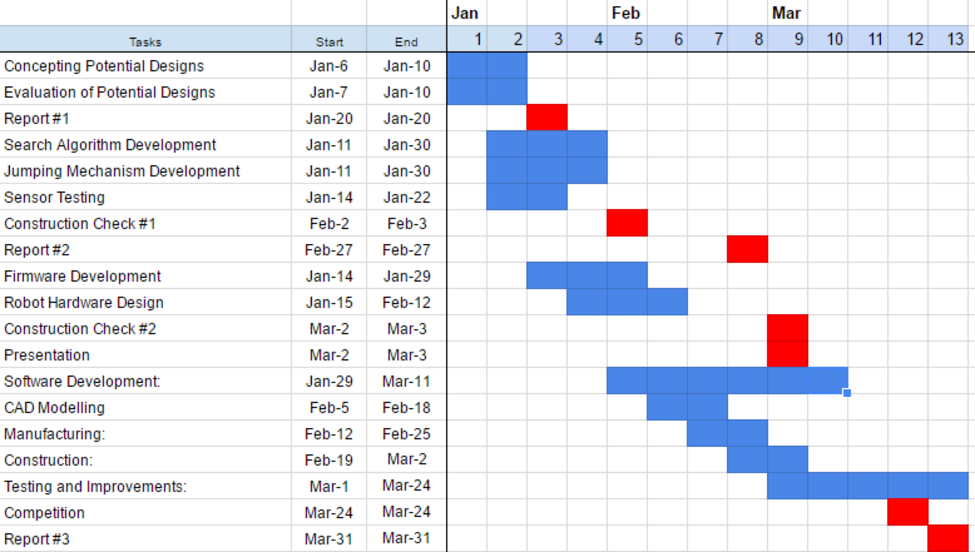
\includegraphics[width=5.5in]{res/gantChart}
    \caption[Gantt chart of the schedule]
          {Gantt chart of the schedule.}
    \label{fig:gantt}
\end{figure}

Overall, even though there were a few delays, the robot was ready for full repeated testing by the third week of March, which allowed for roughly two weeks of further testing and improvement.

\subsection{Budget}

The following section describes the expenditures being made by the team.

\subsubsection{Bill of Material}

The bill of materials from Report 2 had to be revised for the final design, due to replacement of malfunctioning sensors. The detailed bill of materials, with the materials rounded off to an even number and without tax included, can be seen below in Table \ref{tab:billOfMaterials}.

\begin{table}[!htb]
  \centering
    \caption[Bill of Materials]
    {Bill of Materials.}
    \begin{tabular}{ | l | l | }
        \hline
        Material  & \cellcolor{mygray}Cost (CAD)  \\ \hline 
        \cellcolor{mygray} Sensors  & 50 \\ \hline
        \cellcolor{mygray} Chassis Material  & 20 \\ \hline
        \cellcolor{mygray} Motors  & 100 \\ \hline
        \cellcolor{mygray} Battery  & 20 \\ \hline
        \cellcolor{mygray} Wiring  & 10 \\ \hline
        \cellcolor{mygray} Spring  & 15 \\ \hline
        \cellcolor{mygray} Padding/bearing/shafts/gears  & 250 \\ \hline
        \cellcolor{mygray} Wheels  & 20 \\ \hline
        \cellcolor{mygray} Miscellaneous materials (Glue/Tape/Adhesives)  & 30 \\ \hline
        \cellcolor{mygray} Total (CAD)  & 515 \\ \hline
  \end{tabular}
  \label{tab:billOfMaterials}
\end{table}

\subsubsection{Cost analysis}

Based on the bill of materials, it can be clearly seen that majority of the budget (more than 50\%) went into the costs for the padding/bearing/shaft/gears for the robot. This is expected as a key requirement of the system would be to ensure these components can handle high impact loading. The next most expensive component are the driving and latch releasing motors, which were required to have sufficient torque to both release the latching mechanism and to drive the robot. 

\section{Final Mechanical Design} \label{mech}

The following section describes the final mechanical design of the robot as well as how the predicted results compared with real life results.

\subsubsection{Key Modifications}

Many mechanical modifications were needed after unforeseen complications. Such difficulties included but were not limited to: Motor encoders not being protected by the chassis, the robot not jumping high enough, plastic deformation of dimension sensitive components, and mechanical disturbances interfering with driving.  

Figure \ref{fig:mech1} shows how the motor encoders were exposed in the original mechanical design. Without protection they would be prone to breakage since they would either impact the floor or scrape against the ground. It was also determined that the time of flight sensor was not sufficient to find the destination. It was therefore determined that ultrasonic sensors would be used to find the destination. Given the new algorithm, a key requirement was that the sensors point perpendicular to the path of the robot. A naive solution to this problem is to place the sensor as shown in Figure \ref{fig:mech2}. This configuration, however, makes the sensor vulnerable to impact. Thus, combining the issue of motor encoder protection and Ultrasonic sensor placement, the team decided to expand the chassis. This modification is shown in Figure \ref{fig:mech3}. 

\begin{figure}[!htb]
    \centering
    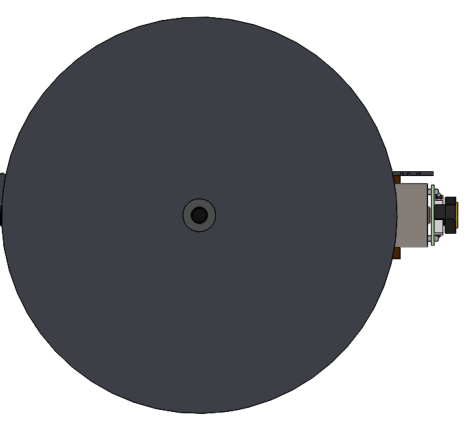
\includegraphics[width=3.5in]{res/mech1}
    \caption[Side-view of the Robot showing the motor encoder]
          {Side-view of the Robot showing the motor encoder sticking out.}
    \label{fig:mech1}
\end{figure}

\break

\begin{figure}[!htb]
    \centering
    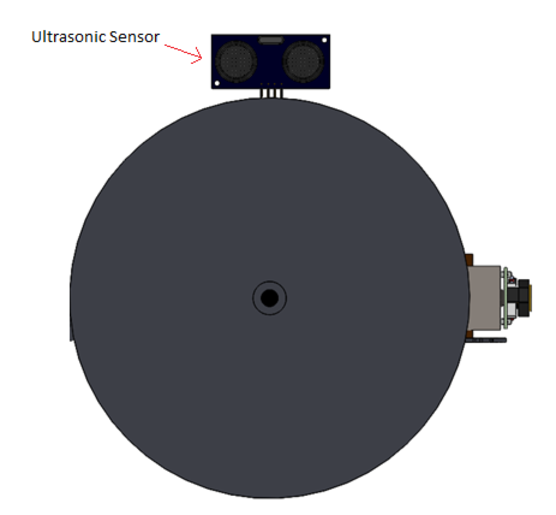
\includegraphics[width=4.5in]{res/mech2}
    \caption[Possible Ultrasonic Sensor Placement]
          {Possible Ultrasonic Sensor Placement.}
    \label{fig:mech2}
\end{figure}

\begin{figure}[!htb]
    \centering
      \captionsetup{justification=centering}
    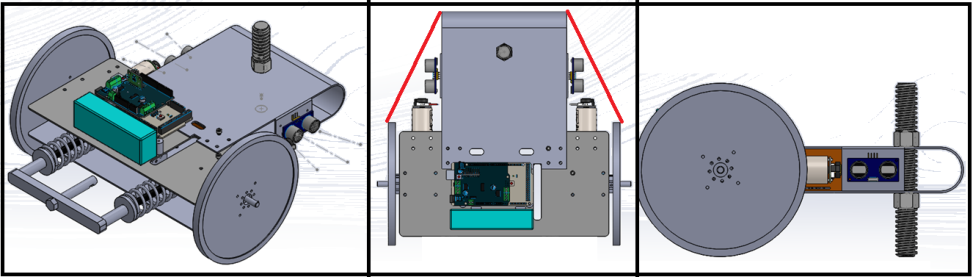
\includegraphics[width=5.5in]{res/mech3}
    \caption[Different views of final design]
          {From left to right: Isometric view of the expanded chassis, Top view showing the robot geometry protects the sensors with the red triangle, Side view of the robot.}
    \label{fig:mech3}
\end{figure}

As seen in Figure \ref{fig:mech3} the sensors are placed such that they are far from the ground. This means it will provide enough space so it will not detect the ground. The new geometry of the robot means that both the encoders and ultrasonic sensors are protected from impact, regardless of the orientation the robot falls in. This also ensures that the ultrasonic sensors are positioned symmetric to the robot in such a way that it will work regardless of the orientation that the robot falls in. The chassis expansion also provided extra real estate to store the payload inside the robot while improving structural integrity.

The second modification was the latching/compression mechanism. One major problem with the previous mechanism was that it was not energy efficient, the actual jumping height was under half the calculated values due to unforeseen mechanical losses. Moreover, the winching motor had failed, thus requiring a more robust solution. The team conceptualized a latching mechanism similar to how doors work, pictured in Figure \ref{fig:mech4}. The notch latches onto a shaft that has two orthogonal flat faces as shown in Figure \ref{fig:mech5}. The system would unlatch as the shaft is actuated/rotated by a DC motor. Nevertheless, this sacrificed a key feature of the robot. The robot was no longer able to compress the springs without assistance and thus is no longer able to jump multiple times without human intervention. Nevertheless, the robustness and energy efficiency of the new system outweighed the sacrifices. Moreover, it prevented possible damage to the motor that might have resulted from releasing the latch since the motor is no longer providing any torque to hold the latch in place. It was more energy efficient as the robot did not have to lift the weight of the jumping mechanism, nor did it damage any components holding the shaft in place. 

\begin{figure}
    \centering
    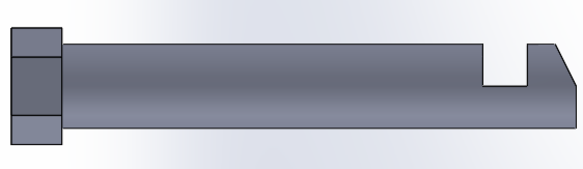
\includegraphics[width=3.0in]{res/mech4}
    \caption[Latching bolt]
          {Latching bolt.}
    \label{fig:mech4}
\end{figure}

\begin{figure}
    \centering
    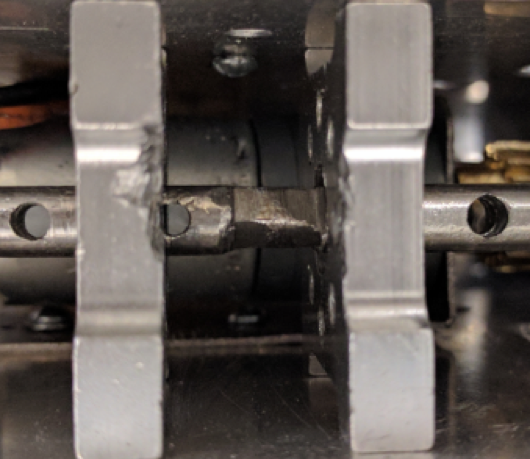
\includegraphics[width=3.0in]{res/mech5}
    \caption[Latching shaft]
          {Latching shaft.}
    \label{fig:mech5}
\end{figure}

After changing the latching mechanism, the team realized the foot was plastically deforming each time the robot was compressed. This would eventually cause brittle failure in the material while more immediately changed the compression distance of the springs. This can be attributed to the fact that the latching bolt significantly reduced the amount of material at the greatest point of stress. Figure \ref{fig:mech6} shows the amount of material resisting bending before the modification. The foot was re-machined to be wider and taller to lessen the bending stress as shown in Figure \ref{fig:mech7}.

\begin{figure}
    \centering
    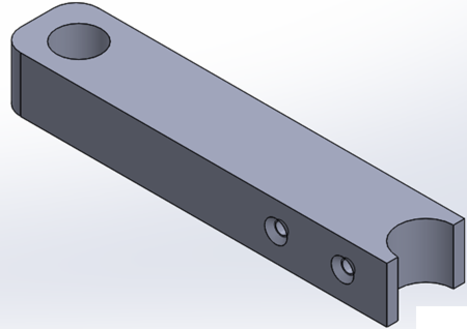
\includegraphics[width=3.0in]{res/mech6}
    \caption[Cross section of the Foot]
          {Cross-Sectional Area of the Foot.}
    \label{fig:mech6}
\end{figure}

\begin{figure}
    \centering
    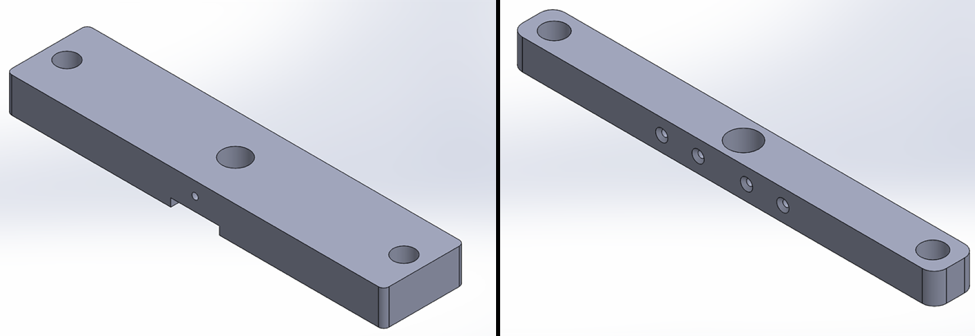
\includegraphics[width=5.5in]{res/mech7}
    \caption[Comparison of changes in mechanical design of foot]
          {New Foot (Left) against Old Foot (Right).}
    \label{fig:mech7}
\end{figure}

Another add-on to the foot is the guiding ski as pictured in Figure \ref{fig:mech8}. The robot needed to drive vertically for the first half of the course to accommodate for the jumping mechanism as shown in Figure \ref{fig:mech9}. This component would provide a 3-point contact with the floor. Since these were machined out of thin aluminum sheet metal plates, two were stacked to increase rigidity. If the foot was not rigid enough the robot would lean too much forward and the Time of Flight sensor could detect the floor. This would lead to a false positive for jumping, which would be disastrous. This component was also used to adjust the jump angle, by bending the part as required as shown in Figure \ref{fig:mech10}. Figure \ref{fig:mech10} also shows how a block of aluminum was attached to the long part of the guiding foot to further increase rigidity. 

\begin{figure}
    \centering
    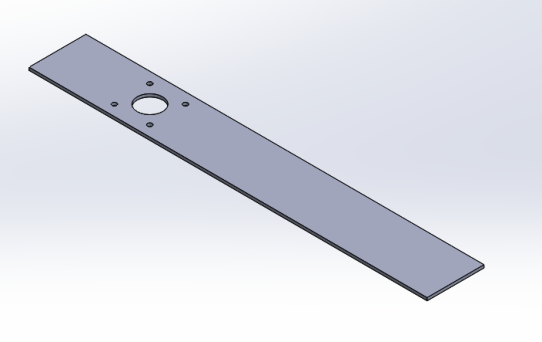
\includegraphics[width=3.0in]{res/mech8}
    \caption[Guiding Foot]
          {Guiding Foot.}
    \label{fig:mech8}
\end{figure}

\begin{figure}
    \centering
    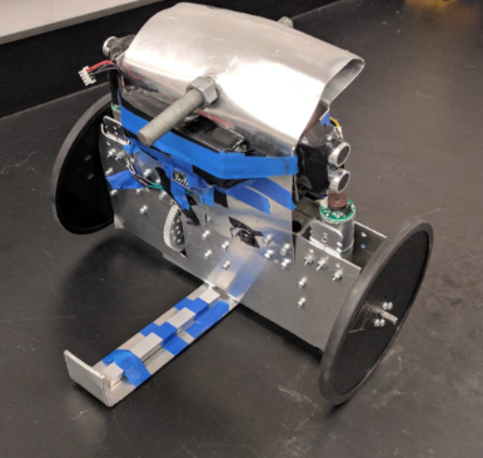
\includegraphics[width=3.0in]{res/mech9}
    \caption[Vertical Driving Configuration]
          {Vertical Driving Configuration.}
    \label{fig:mech9}
\end{figure}

\begin{figure}
    \centering
    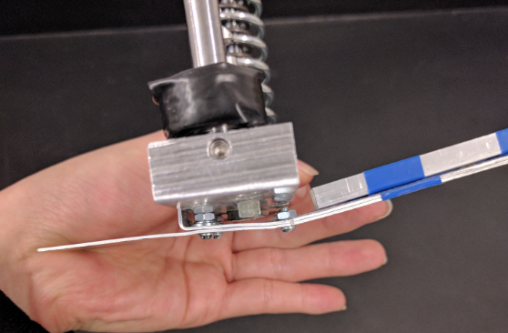
\includegraphics[width=3.0in]{res/mech10}
    \caption[The Bent Guiding Foot]
          {The Bent Guiding Foot.}
    \label{fig:mech10}
\end{figure}

After all the previous modification, the mass of the robot drastically increased, from 1.5 kg to almost 2.6 kg. The previous springs did not store enough energy to clear the 0.9 m wall. The team wanted to devise a solution that required the minimal modification, as a major modification would require significant machining time and testing. Thus, a thinner spring that fit inside the existing spring was inserted in the linear rod. Figure \ref{fig:mech11} shows the darker spring inside the silver spring. This provided enough energy for the robot to clear the wall.

\break

\begin{figure}
    \centering
    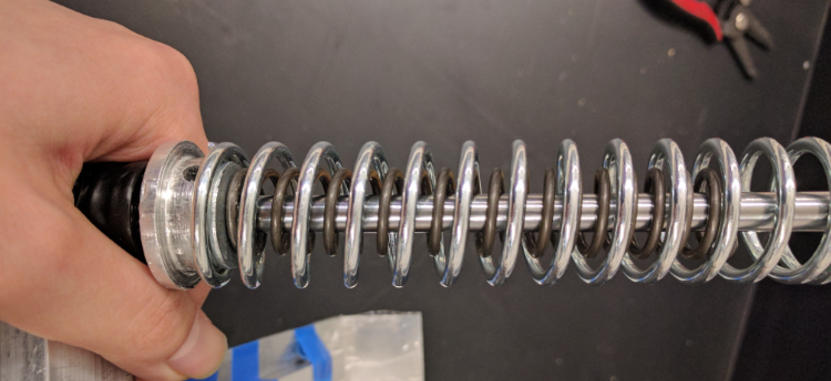
\includegraphics[width=4in]{res/mech11}
    \caption[Parallel Spring Configuration]
          {Parallel Spring Configuration.}
    \label{fig:mech11}
\end{figure}

Lastly, a foam board gate was constructed to aid the robot get off the starting platform. The gate, as pictured in Figure \ref{fig:mech12}, met the dimension requirements and made sure that the guiding foot did not get stuck in the step between the platform and the floor. Furthermore, it also served as a safety mechanism. In the case that the robot unlatches while setting it up in the starting platform, the foam would absorb most of the jumping energy. This proved successful, as one team member was not injured when the robot unlatched during robot alignment. From observation, the robot jumped at most 0.3 (m) and was confined within the platform.

\begin{figure}
    \centering
    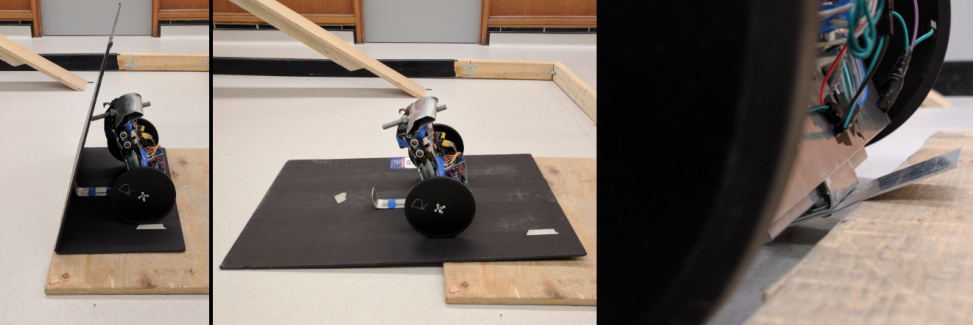
\includegraphics[width=5.5in]{res/mech12}
    \caption[Launch platform]
          {Left to Right: Closed Gate. Opened Gate, and Foot getting stuck on the platform.}
    \label{fig:mech12}
\end{figure}

\subsubsection{Key Features}

The key mechanical feature of the robot is sturdiness. The robot was designed to take multiple impacts equivalent to a 1 m fall. The chassis was built from aluminum sheet metal which provided rigidity but also flexibility so it does not break under impact while absorbing energy. The geometry of the robot also made sure all the electrical components were protected. Although the wheel shafts did noticeably bend, the PID controller was robust enough to make the robot drive at desired directions. At no point during testing, did the mechanical components break, except the plastic bevel gears. Fortunately, the team had extra bevel gears as backup.

Another feature is that the jumping height could easily be adjusted by adding and removing washers to change the compression displacement of the springs. This gives more flexibility in the application of the robot should it be further developed to make it more efficient in the course by jumping earlier and with initial velocity to save time.

\subsubsection{Testing}

The final stages of testing involved running the course in different section. Mechanically, the team wanted to minimize disturbances that would affect robot control, and the robot could withstand repeated impacts from falling and crashing. It was very costly to carry out a full test (start from the platform to finding the pole), as the springs had to be manually compressed and it was physically straining to the designated robot compression member. End to end testing was minimized to reduce wear, and filming from multiple angles prevented the requirement of retesting of the same parameters. 

Overall more than 30 jumping tests were performed. Driving and pole searching tests were carried out until they were perfected. Many issues were discovered during testing. In terms of driving, the guiding foot occasionally got caught on the ground, which affected its ability to drive straight. The team solved this by taping the bottom surface with scotch tape, which made the surface smoother. For jumping, the team adjusted the number of washers added to balance between height and ease of compressibility. 

There was significant plastic deformation in the chassis, the wheel shafts, and the latch. From video analysis, the ABS wheels deflected enough to collide with the chassis and bend it. The chassis scratched the wheels and even pierced the tires. The wheel shafts bend enough, to cause the wheels to wobble while driving. Also, there were several dents and bends in the chassis. Nevertheless, they did not interfere with the performance of the robot. The latch needed filling to make sure the edges were straight, as shown in Figure \ref{fig:mech13}. Overall, the design prevented any significant breaks or deformation saving time and money both from machining and re-ordering parts.

\begin{figure}
    \centering
    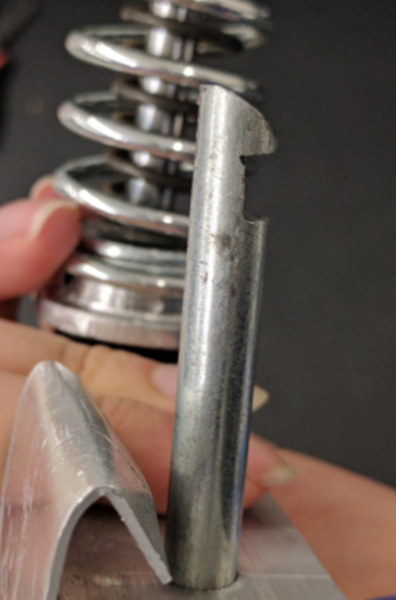
\includegraphics[width=2.0in]{res/mech13}
    \caption[Latch showing wear/tear from usage and filing]
          {Latch showing wear/tear from usage and filing.}
    \label{fig:mech13}
\end{figure}

\subsubsection{Predicted Results Vs. Actual}

In the calculations made in the last report, the wheel shaft was not expected to plastically deform. However, the parameters from the calculations were different from the final robot. One major factor was the mass of the robot, which increased from 1.5 kg to more than 2.5 kg. Thus, the deflection from wheels, chassis, and shafts were greater than expected. Nevertheless, most of the mechanical system did not break during testing. One component that did break was a bevel gear. A tooth broke off of the gear during testing which caused skipping while driving. However, the problem was easily solved as replacement parts were available. In the previous report, the safety factor for the bevel gears was 1.5 for driving conditions. However, the team suspects that the gear broke because the team did not consider how the chassis flex stresses the wheel/driving mechanism or additional torque while landing.

\subsubsection{Lessons Learned}

There were several lessons learned during this project. Firstly, switching mechanism designs halfway through development of the robot brings a plethora of new problems. Since mechanical components are interconnected and affect each other, one change is usually followed by many other modifications. Thus, it is better mechanical design practice to foresee as many problems as possible before designing and manufacturing the final product. The team also realized the machining limitations brought issues in the final construction. Misaligned holes made it impossible to align the drive gears. Thus, the mating would not be perfect, which meant that a controller was vital for driving. 

There were many last-minute fixes to the mechanical design as seen in Figure \ref{fig:mech9}. As seen, the robot is covered with electrical tape and looks unprofessional. This has taught the team the importance of more rigorous early testing so that things do not break last minute. 

Overall, the mechanical system was robust enough to prevent breakage. Nevertheless, a better job could have been done to improve the robot’s performance in terms of weight reduction and controllability. 

\section{Final Electrical Design} \label{electrical}

The following section will describe the general electrical design from a high level and key components that may have change since the second report. 

\subsection{General Electrical Design}

In terms of the general electrical design, comparing to the detailed design report submitted as Report \#2, there was a few changes, with the primary one being that a Time of Flight (TOF) sensor was added. On the final design of the robot, different pins are used for a lot of the components to ease construction. Below, in Figure \ref{fig:wiring}, the electrical wiring diagram of the robot is displayed. 

\begin{figure}
    \centering
    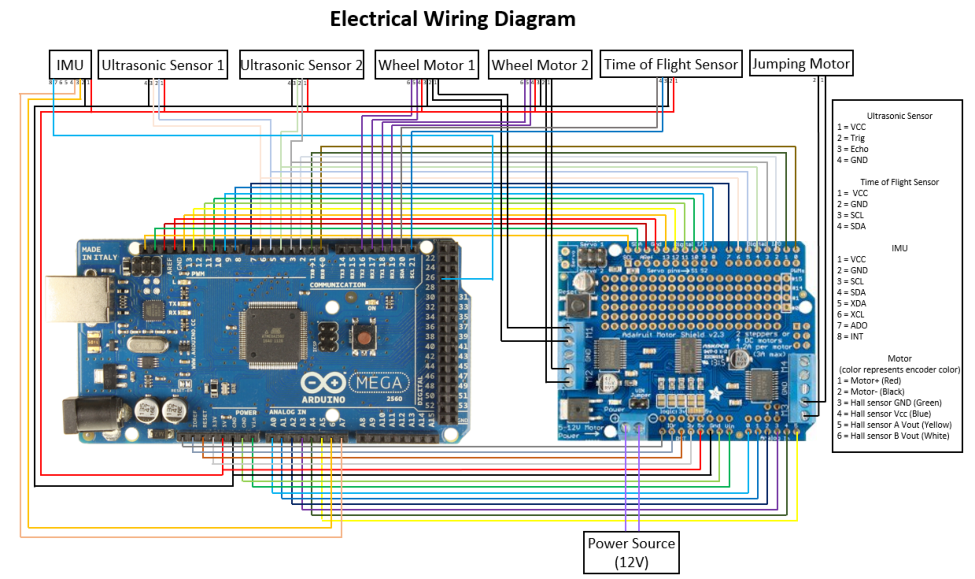
\includegraphics[width=5.5in]{res/wiringDiagram}
    \caption[Arduino wiring diagram]
          {Arduino wiring diagram.}
    \label{fig:wiring}
\end{figure}

\subsubsection{Key Features}

Due to the relatively low complexity of the electrical design for the robot, the main objective of the electrical design is for low assembly complexity and ease of cable management. The wires were glued to the pins to prevent disconnection while testing the jumping and impact capabilities.

\subsubsection{Design Exploration} 

Initially the robot was assembled according to the electrical wiring diagram as shown in report \#2. However, it was quickly seen that there was a large amount of wires which are simply plugged into the Arduino board. Due to this, changes were made to move some of the pins to the motor shield connections, which would allow the team to solder the connections directly to the board, reducing the risk of disconnecting while landing. As such, through the course of robot assembly and construction, the wiring diagrams were changed and the final result as seen in Figure \ref{fig:wiring} above.

\subsubsection{Testing} 

As testing of the robot commenced, it was observed that the friction provided by the mechanical connections was not sufficient to prevent disconnection. Steps were taken to strengthen the common connections. As such, the connections were all soldered together, then electrical tape was used to insulate against potential shorting. In some cases, electrical tape was used to secure the connections to the sensors, to ensure they will not become unplugged. Glue was also used as a removable but secure method of fastening.

\subsubsection{Predicted Results Vs. Actual} 

Overall few modifications were required, testing mainly revealed that further fastening was required to ensure system stability.

\subsubsection{Lessons Learned}

Through working on the electrical design, several lessons were observed. The first is that even though the complexity of the actual electrical circuits was low, there are still several key functionality issues, ranging from how the connections will perform against shock and chances of short-circuits. The first point was observed several times, where strange behavior was a result of poor connection from a sensor being unplugged. As such, the electrical design needs to be done in such a way that after impact the connections can still be trusted. 

\section{Final Control Design} \label{controls}

This section will provide a detailed overview of the final implementation of the robot control architecture. When compared to the previous report, the changes have mainly involved the controller design as well as the finalization of the pole location algorithm.

\subsection{Robot Position and Velocity Control}
The overall design of the Robot's position and velocity controller has changed to better consider external disturbances that original in the mechanical design. Originally, the design called for two PID controllers driving each of the wheels individually as shown in Figure \ref{fig:singleWheelController}. 

\begin{figure}
    \centering
    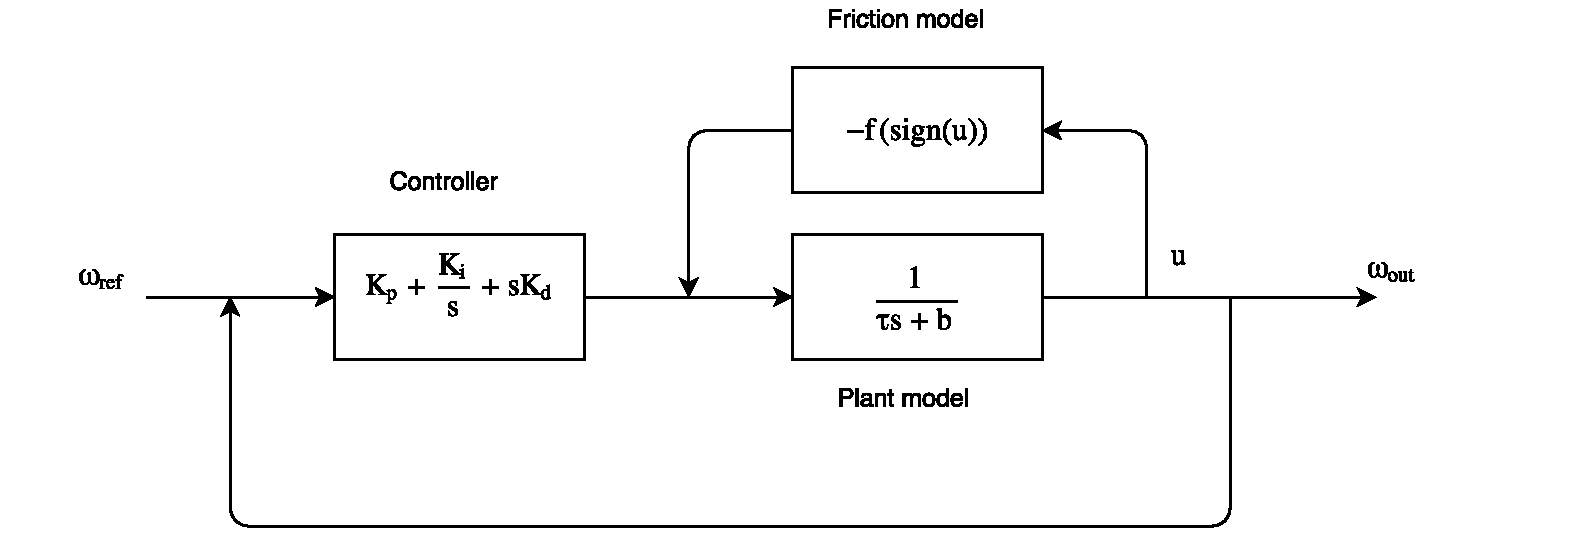
\includegraphics[width=5.5in]{res/380ModelForWheel}
    \caption[Controller for an individual Wheel]
          {Controller for an individual Wheel.}
    \label{fig:singleWheelController}
\end{figure}

The individual speed where determined through kinematic equations related individual wheel speeds to the robot's overall speed and angular velocity. Figure \ref{fig:kinematicModel} shows the kinematic model of the robot. Specifically, r describes the radius of curvature of the path, L the length of the robot, $\omega_l, \omega_r$ describes the rotation rate of the left and right wheel respectively. $V_l, V_r$ describe the linear velocities of each of the wheels. R is the radius of the wheels and $\theta$ describes the rotation about the origin. 

\begin{figure}
    \centering
    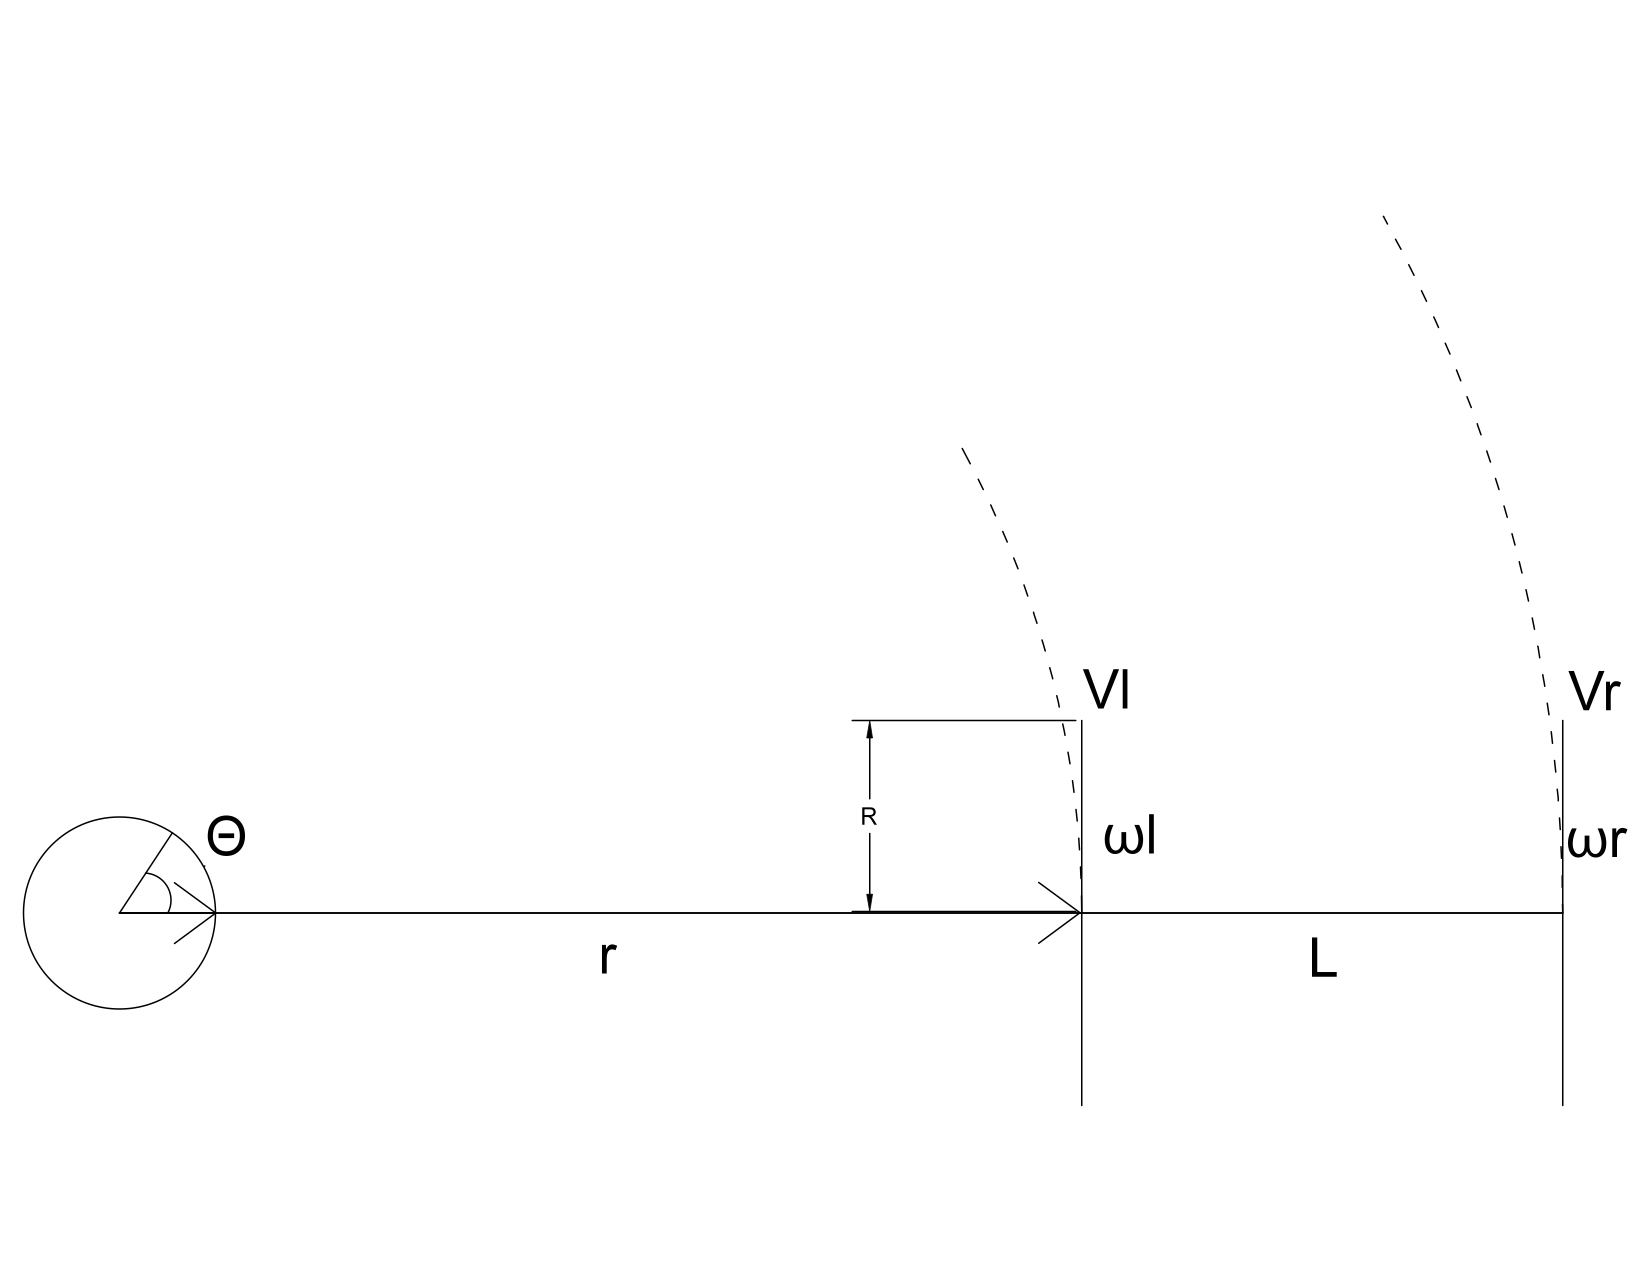
\includegraphics[width=5.5in]{res/diagram}
    \caption[Kinematic model of the robot]
          {Kinematic model of the robot.}
    \label{fig:kinematicModel}
\end{figure}

With this model the following equations can be derived, full details are found in the previous report. V and $\omega$ describe the global tangential and rotational velocities desired. It is important to note the assumptions that were made to obtain these results. Mainly, that no slip exists between the wheels and the ground, and that all components within the drive train are always in contact, hence ignoring the backlash.

\[\omega_l = \frac{2V-\omega L}{2R},\omega_r = \frac{2V+\omega L}{2R}\]
\[V=\frac{R}{2}(\omega_l+\omega_r),  \omega=\frac{R}{L}(\omega_r-\omega_l)\]

It was assumed if the wheels were individually capable of maintaining its speed, the robot overall would be able to follow a straight track accurately. However, this left the issue that the true variable that was desired to be controller was open loop, and error from either motor in terms of speed would result in the integration of error. The process that was used to overcome this issue is described below.

\subsubsection{Design Exploration}

During initial testing, it was difficult to achieve straight line driving on the platform. Through analysis of the individual wheel's speed over time, it was determined that while on average the individual speed's were very similar, biases existed due to disturbances from construction. There are multiple root causes for this: differing alignment on bevel gears, imperfect shafts, and differing motor characteristics. Overall, this caused significant turning while driving in a straight line.

A key observation made is up to this point, the yaw of the robot is controlled in open loop. The obvious solution to this is to implement another controller around the yaw of the robot. Firstly, the following equation was derived through integration with a zero initial condition assumption.

\[\theta_r = \int\omega_rdt\]
\[\theta_l = \int\omega_ldt\]
\[\theta=\frac{R}{L}(\theta_r-\theta_l)\]

Given that there is a measure of the current angle, a PID controller can be defined to ensure that the desired angle is being outputted. The block diagram of the model is described in Figure \ref{fig:yawController}.

\begin{figure}
    \centering
    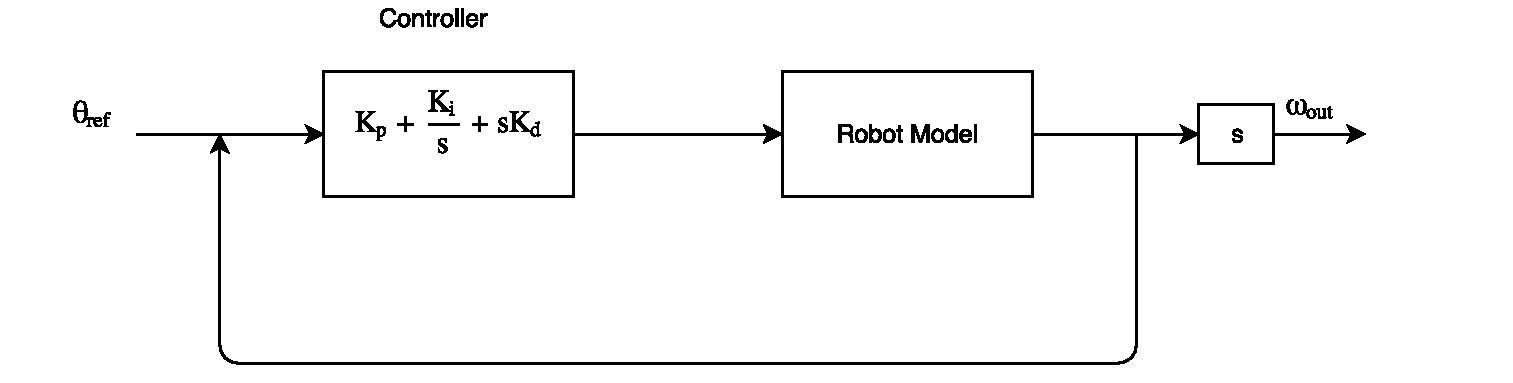
\includegraphics[width=5.5in]{res/yawController}
    \caption[Robot yaw controller]
          {Robot yaw controller.}
    \label{fig:yawController}
\end{figure}

Given the correction rotation rate as the output of the controller, corrections to the yaw can be made by changing the desired yaw being used to calculate the individual wheel speeds. In order to maintain generality, the reference angle is defined as follows where $\Delta t$ is the time step between updates. 

\[\theta_{ref} = \sum\omega \Delta t\]

This ensures that the robot achieves an angle as if it were following the desired rate of rotation over time. It is important to note that the kinematic model decouples the tangential and rotational velocities, which allowed for minimal change to the previous implementation. 

During testing, the same tuning of the controller parameters was unable to achieve stability in both the jumping and pole searching orientations of the robot. To combat this a gain schedule was implemented to adaptively change the tuning based on the orientation of the robot. 

\subsubsection{Key Features}

By using the full kinematic model of the system, it is possible to control both the speed as well as the angular velocity of the robot through a simple interface. Moreover, since any path can be generated using a tangential and angular velocity, the implemented design is theoretically capable of physically replicating any desired trajectory with little development effort. Given the modifications, and a full model of the system, theoretical guarantees can be made about the accuracy of the position of the robot at any time. However, it is important that all times the assumptions of the system must remain valid otherwise significant tracking error will occur as described later.

\subsubsection{Testing}

During end to end testing of the robot the assumptions that were made to formulate the controller were strained. One of the first issues that was noticed was that after impact from landing, there was a possibility that the bevel gears within the robot were decoupled from their shafts. That is, the torque being transferred from the motor was not reaching the wheels themselves. However, the issue presented itself as one wheel spinning slower than the other, which resulted in confusion, and doubt in the controller implementation. Moreover, when the orientation of the robot in the jumping state, there were instances where the wheel did not touch the ground resulting in the robot spinning in place. These issues show the sensitivity of the algorithm to the initial assumptions that were made. Without moving the encoders to measure the output shaft or purchasing an accurate IMU to measure the overall yaw, these issues cannot be solved in software. 

Another result that was found from testing, is that when immediately commanding the motors to drive at a high speed, there was a high transient error that would not be corrected for in the length of the course ($<2$ (m)). However, this error did not exist at low speed. This lead to the conclusion that a velocity profile would act as the simplest solution to prevent any error from existing. While this was the implemented solution, it is important to note that the yaw controller itself was tuned for somewhat slower response to minimize oscillation. By increasing the performance of the controller, it would be possible to achieve a better overall response with a much faster ramp up time. 

A final experiment indicated that the overall system could position the robot better than 1 (cm) accuracy in terms of distance. Along with the high rotational accuracy, this meant that the half of the course before jumping over the wall was largely a function of human placement. Barring an orientation algorithm against the wall before jumping, localization within the course was not feasible and therefore not pursued. This prevented perfect pose within the course at all times, which presented itself during the competition when the above assumptions were violated. 

Another key victory of the design was that the robot achievied the above results with significantly damaged wheel shafts. The ends of the wheels had large horizontal displacement which would have presented as large disturbances to the controller. It is likely that because the selected tuning for the controllers were not aggressive the system was less sensitive to these disturbances and remained stable and accurate.

\subsubsection{Lessons Learned}

One of the key lessons learned from the implementation described is to ensure that the overall design is less susceptible to measurement errors. In this case, by either using an IMU to measure the pose, or by having the measurement done on the output, the described controller could have prevented many of the issues that took several hours of debugging. Alternatively, by implementing localization code on the robot it would have been possible to achieve the same result without having to change the robot physically. However, this is prohibitive given the limitations of the Arduino mega. 

In terms of control, a key take-away is that different orientation can cause significant dynamic changes to the system and that significantly differing gains are required for stability. 

Lastly, while the described system achieves high accuracy and robustness, a large amount of time was devoted to tuning the controllers to achieve these results. That is, a better method of tuning, perhaps by using the serial to set the tuning values real time would be beneficial. 

\subsection{Pole Location Algorithm}

The following section outlines the development process of the pole searching algorithm which is employed after the robot lands on the destination side of the wall. It defines the constraints and assumptions made to characterize the problem, and the various solutions formulated. 

\subsubsection{Key Features}

The pole searching algorithm is divided into two stages: localization and searching. The localization portion is executed upon landing, and seeks to locate some feature of the course to use as a reference point. This is necessary as the pose of the robot after landing is non-deterministic. Once the robot has localized itself, it performs the destination searching algorithm. 

\paragraph{Localization}

The localizing routine begins by turning the robot on the spot while continuously reading the distance measured by the left ultrasonic sensor. The rotation continues until a minimum in measured distance is detected (characterized by decreasing values followed by increasing values). At the distance minima, the robot is parallel to feature that is being minimized against. With this knowledge, the robot can then drive parallel to the feature using it as a reference, or execute a 90 degrees right turn to drive perpendicular to the feature. The search algorithm requires that the robot be perpendicular to the wall, so it executes the turn and drives backwards by the minimized distance to survey the area between its landing position and the wall, as well as to square itself with the wall using the bumper. 

It is ideal for the robot to localize to the wall, but the on-board sensors cannot distinguish between features of the course, namely the wall, boundary, and ramp. Thus, the algorithm utilizes the assumptions that the robot will land within a certain distance of the wall, and that it will land closer to the wall than any other feature. The ultrasonic distance minimization routine described above will only conclude when the minima found is under a certain threshold distance (0.5 m chosen from tests) to prevent localizing to a feature in the distance, such as the boundary or ramp. This threshold distance increases incrementally with each full rotation so that the robot will eventually localize to some feature if it were to land further than expected. 

\paragraph{Search}

The robot enters the search routine once it is perpendicular to the wall. The search algorithm relies on the assumption that the robot will land close to the ramp, and thus the pole will either be in front or to the left of the robot. The robot drives forward while continuously checking the left ultrasonic sensor for a change in distance larger than a detection threshold (0.3 m chosen from tests). Specifically, the algorithm looks for a “falling edge”, or decrease in distance, which would signify a change from the boundary to pole. To prevent false reading outside the course boundary, a noise ceiling is implemented to reject any measurements greater than the possible distance between the robot and the boundaries (1.7 m chosen from tests). Figure \ref{fig:SAEX1} shows two example scenarios of the robot finding and arriving at the pole using this algorithm.

\begin{figure}[!tbp]
  \centering
  \captionsetup{justification=centering}

  \begin{minipage}[b]{0.4\textwidth}
    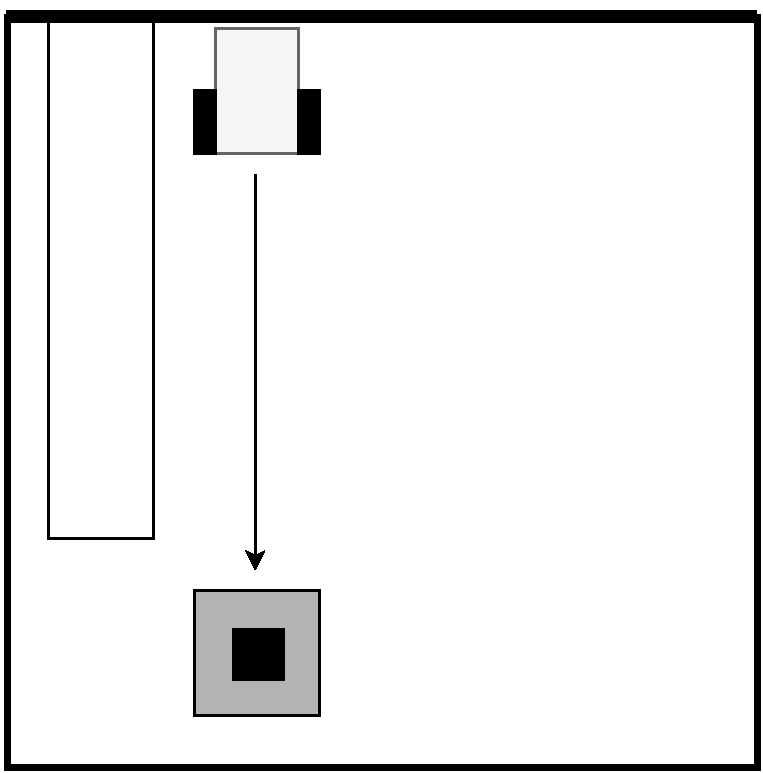
\includegraphics[width=\textwidth]{res/SA-example1}
  \end{minipage}
  \hfill
  \begin{minipage}[b]{0.4\textwidth}
    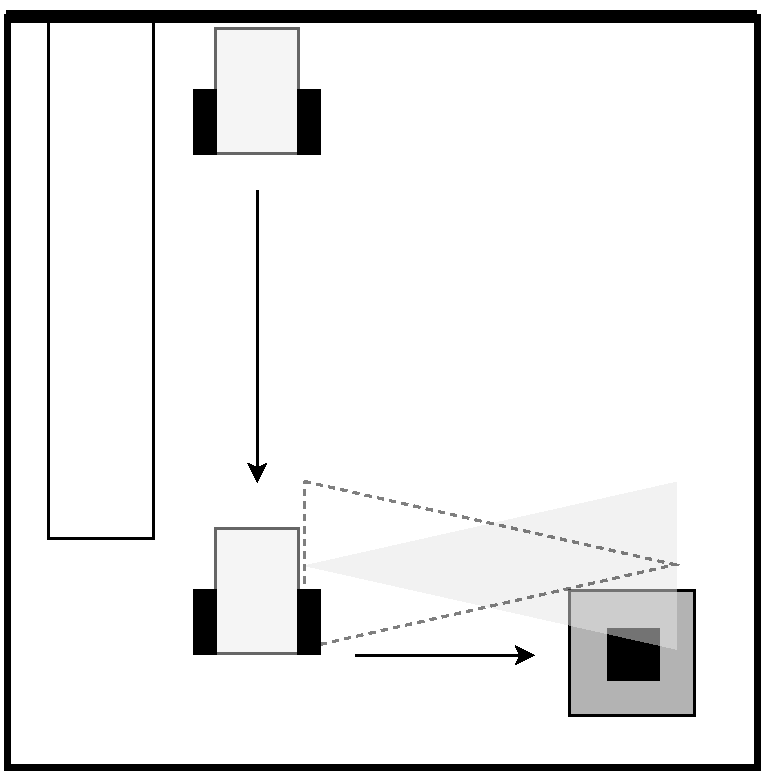
\includegraphics[width=\textwidth]{res/SA-example2}
  \end{minipage}
\caption[Example scenarios of pole detection]{Example scenarios of pole detection. The left figure shows the trivial case where the pole is directly in front of the robot. The right figure shows the general detection process.}
\label{fig:SAEX1}

\end{figure}

Although this algorithm heavily depends on previously having localized to the wall, it is still capable of detecting the pole in some other cases. For example, even if the robot were to drive perpendicularly to the right boundary, it would still be able to detect the pole, as shown in Figure \ref{fig:SAEX3} below. In general, as long as the pole is to the left of the robot, this search algorithm will succeed.

\begin{figure}
    \centering
    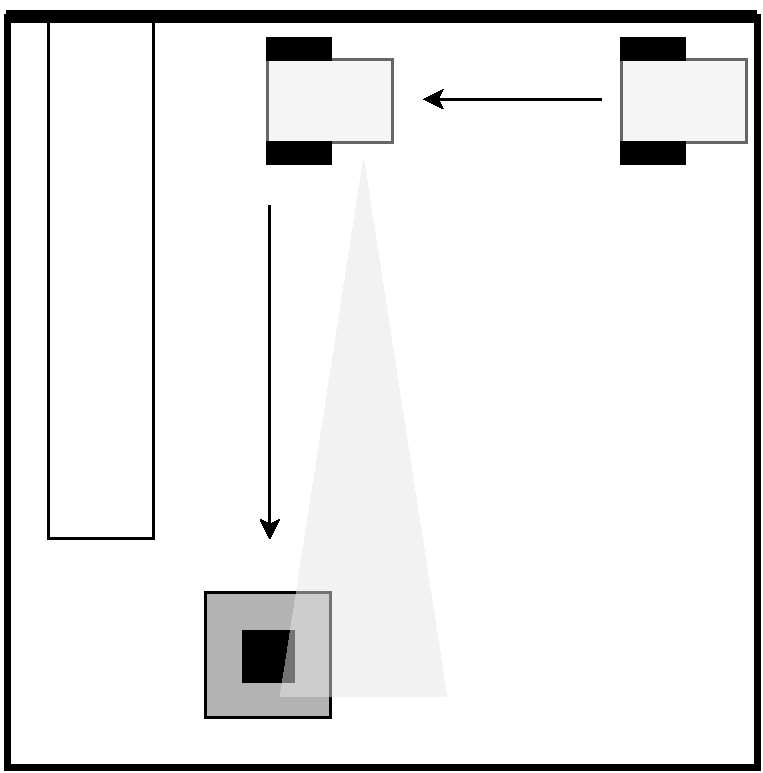
\includegraphics[width=3in]{res/SA-example3}
    \caption[Pole detection from right boundary]
          {Pole detection process in the case that the robot localized to the right boundary.}
    \label{fig:SAEX3}
\end{figure}

\paragraph{Sensor Filtering and False Positive Prevention}

Through testing, it was discovered that the ultrasonic sensor, although relatively precise, occasionally produced wrong values. The incorrect measurement values never appeared consecutively, but posed a threat of causing false positives nonetheless. Two measures were employed combat this issue. Firstly, a running median filter with a window size of three sanitizes the measurement values. In the case of a potential detection of the pole, five additional measurements are made and compared to the triggering measurement with a small tolerance to ensure initial measurement was valid. To lower the chance of a false negative, these confirmations checks have a failure tolerance; two out of five confirmation checks can fail and still confirm the detection.

\subsubsection{Design Exploration}

The pole searching problem was initially divided into the two smaller problems of localization and searching. Although the latter was trivial, the former proved to be difficult enough to be considered a problem on its own. This is largely due to the previous overestimation of the accuracy of the Inertia Measurement Unit (IMU), specifically its ability to measure yaw. Originally, localization was meant to use a reference yaw sampled before jumping to determine the direction perpendicular to the wall. In practice, the yaw measurement of the IMU can drift more than 20 to 30 degrees during the jump, and is unusable. 

For this reason, the team began exploring alternative solutions to localizing the robot. Due to the large area of possible landing locations and different landing orientations, a reliable and general localization method seemed unlikely. Thus, the team decided to explore two high-level concepts in parallel to quickly arrive at a solution. One concept is to constrain the localization problem using assumptions, and fulfill those assumptions by making improvements on other aspect of the robot’s operations (e.g. more consistent jumps and landing area). The second concept is to develop a generalized search algorithm that does not require localization and can distinguish the pole from other course features. 

\paragraph{Constrained Search Algorithm}

The main assumptions which the constrained search algorithm operates under are that the robot will land near the wall and ramp, and that it will land closer to the wall than any other course features. Under this premise, the wall can be differentiated from other course features by scanning for the closest object using the ultrasonic sensor. Given that the jump trajectory was designed with minimum horizontal velocity to maximize height, the robot was also assumed to land within a certain distance of the wall. This distance is used as a second constraint to ensure that the robot localizes specifically to the wall. Although these assumptions are not always correct, there are tangible means to improve their validity by improving the reliability of the jump.

Operating under these assumptions, the localization routine turns the robot in place while scanning using the left ultrasonic sensor. The wall is identified and becomes parallel with the robot when a minimum in measured distance under a limit is found. The limit was implemented to prevent false detection in the case of a corner, which would also produce a minimum. Since the robot is not assumed to be adjacent to the wall upon landing, it then turns 90 degrees to the right to back up perpendicularly to the wall by the measured minimum distance. This allows the robot to square itself with the wall using its bumper to ensure its perpendicularity, as well as ensure that the robot is able to cover the whole course. At this point, the robot is considered localized, and should be perpendicular and touching the wall.  

The search routine uses the same ultrasonic sensor to continuously measure distance while driving away from the wall, parallel to the ramp. This action assumes that the robot lands near the ramp, and thus the pole can only be in front or to the left of the robot. In the trivial case that the pole is in front of the robot, the robot will collide with the pole (highly likely given the large width of the robot). If the pole was to the left of the robot, it would be detected by the ultrasonic sensor. The robot would turn and drive by the detection distance and stop. Combined, the two cases cover the entire possible domain in which the pole could exist at, as shown in Figure \ref{fig:SAAreas}. 

\begin{figure}
    \centering
    \includegraphics[width=3in]{res/SA-Areas}
    \caption[Areas and methods in which each case would detect and arrive at the pole]
          {Areas and methods in which each case would detect and arrive at the pole.}
    \label{fig:SAAreas}
\end{figure}

To increase the robustness of constrained search algorithm as much as possible, several additional measures were implemented to combat pitfalls discovered during testing. For example, the robot will assign left and right ultrasonic sensors and drive direction according to its landing orientation, so that pole searching will still function correctly even if it landed upside-down. In addition, the localization distance limit will also increase with rotations if the robot did not detect anything in range in its first rotation. This is to combat the cases where it lands outside of initial localization range and thus rotates continuously, unable to find a target to localize to. Although this introduces a risk that the robot will localize to some course feature that is not the wall, it guarantees that the robot will localize to something and thus have a chance at finding the pole. 

\paragraph{Generalized Search Algorithm}

During testing, there were several landing cases which indicated a constrained search algorithm may not be sufficient. This was discovered in one of the various jump tests. To combat this a general destination searching algorithm was also implemented. However, after many trials, it was determined that the probability of landing outside of the desired area was low, and therefore the complexity of the general algorithm was unjustified.

In terms of implementing the general search algorithm, several approaches were explored. The first is to align the robot with a corner of the landing zone by having the robot go straight for a set amount of time, turning 90 degrees, going straight for another set amount of time allowing for the robot to align itself with the wall. At this point, the robot will turn 90 degrees, it will then follow the wall by measuring distance to search for the pole. However, with this approach, there are several cases which need to be considered. For example, the corner the robot drives to, and its orientation with the corner. 

Another approach is to have the robot turn in place until the pole is found. At this point, the robot will turn 90 degrees and go straight to the pole. 

Further testing showed that the second approach is the better option. Using the boundaries to align the robot requires significant torque and therefore may damage the robot mechanically. The searching of the pole in one place is a difficult problem, as the ultrasonic sensors have a 30$^{\circ}$ cone of detection, and at large distances the pole may appear as noise. As such a modified version of the localization algorithm is used. It is designed to detect all local minimums in the scanned area. The local minimums will be counted as a pole depending on defined tolerances and conditions. It was determined that this method required significant tuning to ensure reliability. Moreover, several different filters required to be implemented and tested. Overall, given that this is a classification task, a machine learning algorithm would be well suited due to the ease of implementation. However, such algorithms are not feasible due to time and computation constraints.

\subsubsection{Testing}

Testing for the individual search algorithms was conducted by placing the robot at an ideal starting position, and running through the routine. A reliability test is first conducted by running ten trials of pole searching with the pole kept in the same place. This ensures that the algorithm operates consistently and that correct detections are not circumstantial. Then, the implementations are tested using edge and corner cases. This includes detecting the pole at the extremes of possible locations (far and near corners of the course), and detecting the pole while upside-down. Once an algorithm was deemed reliable inside expected operating parameters, it is tried in extraneous to determine limits of reliability. 

\subsubsection{Predicted Results Vs. Actual}

The constrained search algorithm was initially predicted to be unreliable, and was only explored as it was viable within time constraints. However, in testing, the algorithm worked almost infallibly under the constrained conditions. Specifically, the localization routine correctly identified the wall consistently, which gave the robot a solid starting point to conduct searching. The searching routine, despite being simpler in operation, was the most common cause of failure in pole searching. Both false positives and negatives were prevalent (the former more than the latter). Additional filtering and confirmation checks were implemented in response, resulting in an increase in reliability to acceptable levels (9 out of 10 success rate). 

In addition, while testing the constrained search algorithm with extraneous landing locations, it was discovered that the algorithm still works even if the robot were to localize to the right boundary. This is due to fact that the algorithm searches for the pole on the left side of the robot. If the robot were to drive perpendicular to the right boundary, the majority of the course area is still to its left, and thus the algorithm would still function. The chances of successful pole search based on landing location is shown in Figure \ref{fig:SAdetection}. The areas of high chance of detection corresponds to areas with high chance of localizing to the wall or right boundary, with majority of the course area to the left. Landing in the moderate chance of detection area gives the robot a chance to localize to either the wall or right boundary, but the outcome is ambiguous.  

\begin{figure}
    \centering
    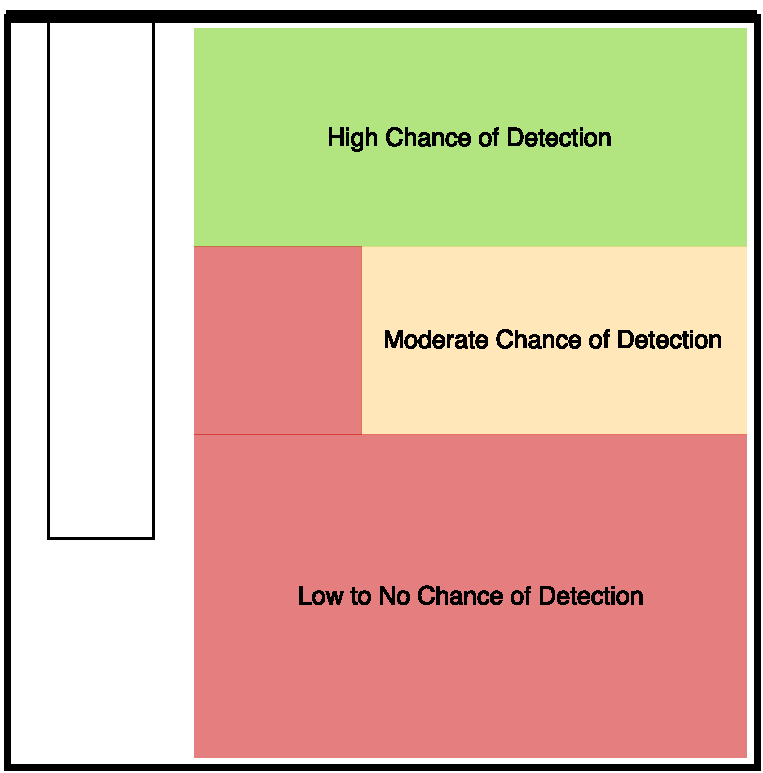
\includegraphics[width=3in]{res/SA-areaofdetection}
    \caption[Probability of successful pole search based on landing position]
          {Probability of successful pole search based on landing position.}
    \label{fig:SAdetection}
\end{figure}

In terms of the general search algorithm, initial testing shows promise. However, there were a several of false detections which could be tuned out. Given the difficulty of tuning as well as the low initial reliability as compared to the constrained algorithm, the generalized algorithm was not used.

\subsubsection{Lessons Learned}

Firstly, the team learned that sensors are unreliable. If the IMU operated as expected, then much of these considerations would not have been necessary. Even in the case of the ultrasonic sensors, moderate filtering was required for reliable data. Realistically, to develop a robust search algorithm, the algorithm must accommodate the shortcomings of the sensors. At the same time, precautions can be taken to increase sensor reliability. A compromise in the middle is ideal.

The process of developing these search algorithms also gave the team practice in breaking down problems. Although initially daunting, a reliable pole searching algorithm was eventually made possible by scaling down the problems and making reasonable assumptions. The overall problem can then be solved by either scaling up the solution to a smaller problem, or by fulfilling the assumptions made. This framework is applicable to many real-world engineering problems, and may be crucial to reaching their solutions. 

\section{Competition Result Analysis}

There were many differences and unforeseen challenges during the competition. Although this was expected, there were more problems than anticipated. One of the issues that took most of the debugging time was the jump mechanism. The jumping mechanism was not as robust as initially believed and as such required modification. One of the biggest challenges was that the testing time and risk were lot higher than other designs. It was noted that the more jump tests marked a notable decrease in system reliability. Moreover, these jump tests uncovered several simple problems but time consuming problems such as wiring disconnections.

The second challenge was the tuning for the controller. Since the robot has two states, the team had to tune controllers for both. One of the main issues was that modifications to the jumping mechanism may require retuning of the system. Also, there was the possibility that a poor landing may result in a poorly tuned controller.

The completion time of the robot was longer than expected mainly because the jumping state of the robot was effectively an inverted pendulum. Every transition needed some time delay for the dynamics to decay to prevent assumptions made in the controller from being violated. This had put a huge constraint on time but made the controls more manageable since the team could work on separate parts of the state while the assuming of zero initial conditions or assuming that the dynamics from the previous states were negligible.

Overall, although the robot’s performance was worse than expected, the course was still completed with the jumping approach. This was the primary goal of the team. Knowing that in the three years of the competition that there has never been a successful jumping robot, the fact that the robot successfully completed the course is a great result. 

\section{Conclusions}

This report provided an overview of the robot that was designed to be capable to delivering aid to individuals trapped within unsafe territory autonomously. An analysis was presented of the constraints that are present within the environment and how the presented design overcomes them. By using the components and testing the validation of the mechanisms, allowed for design review, modification, and optimization of the robot. 

The time-line of the project was examined, and the changes that were required in the schedule were presented and discussed. Moreover, the final bill of materials is examined along with a cost analysis of all components. Overall, the project came in at a cost of around 500 Canadian dollars, and took 12 weeks to complete. 

Implementation details, involving mechanical, electrical and controls were presented and their respective advantages and disadvantages are discussed. An overview of how the jumping mechanism changed over design period was presented. Moreover, the details of mechanically protecting the robot were also shown. Details involving the minimal changes electrically were shown. In terms of control, the final control scheme was presented and analyzed. Moreover, the theoretical guarantees of the implemented search algorithms were discussed while providing statistical analysis its performance. 

A comprehensive review of the performance and the reasoning behind it is presented. This involved looking back at issues that were inherit to the design, as well as defining better engineering practices. Tuning was highlighted as a major issue both in the case of jumping and driving the vehicle. Finally, the results of the competition are determined to be a success due to the completion of the course with a novel design. 

% \section{Fourth Year Design Project Proposal}

% The following section describes the proposal of the fourth year design project. It defines the constraints and criteria of the design, which resulted in a decision to create a robot capable of making sandwiches using custom CNC assembly line.

% \subsection{General Background}

% Many people today work at fast food places with their job mainly being assembling sandwiches. There have been many efforts to automate this process but to bring people fresh and clean sandwiches has always been a challenge. There is an increase of amount of people seeking for quick and easy solution to their meal problem during a busy day.

% \subsection{Needs assessment}

% The need to combat the demand for fast food and lower price is clear. Fast food companies are offering incredibly cheap food but to offer even cheaper and faster service, a method to be able to automate the construction of fast food sandwiches are in high demand.

% \subsection{Problem Formulation}

% Problem that is in need of a solution is to automate the sandwich making process.

% \subsubsection{Problem definition}

% Design a device to quickly and safely make fast food sandwiches.

% \subsubsection{Desired functions and goals}

% The main function of the device is to assemble few different sandwiches from some fast food restaurants. The goal is to assemble the sandwiches faster than a human worker with higher reliability and contamination free quality.

% \subsubsection{Constraints}

% The device must autonomously assemble the sandwiches. It must operate safely along human workers.  The device must be able to replicate the sandwiches that it assembled.

% \subsubsection{Objectives}
% The device should take less than a minute to assemble one order. The operating cost should be less than the minimum wage per hour. The device should be IP65 rating.

%%%%%%%%%%%%%%%%%%%%%%%%%%%%%%%%%%%%%%%%%%%%%%%%%%%%%%%%%%%%%%%%%%%%%
%% BACK MATTER
%%%%%%%%%%%%%%%%%%%%%%%%%%%%%%%%%%%%%%%%%%%%%%%%%%%%%%%%%%%%%%%%%%%%%
% \begingroup
% \raggedright
% \sloppy
% \bibliography{uw-wkrpt-bib}
% \endgroup

%%%%%%%%%%%%%%%%%%%%%%%%%%%%%%%%%%%%%%%%%%%%%%%%%%%%%%%%%%%%%%%%%%%%%
%% APPENDICES
%%%%%%%%%%%%%%%%%%%%%%%%%%%%%%%%%%%%%%%%%%%%%%%%%%%%%%%%%%%%%%%%%%%%%
\appendix

\end{document}